\chapter{Connections to $S_n$}\label{chap:connections-to-sn}
\epigraph{till Max said ``BE STILL!''\\
  and tamed them with the magic trick\\
  of staring into all their yellow eyes without blinking once\\
  and they were frightened and called him the most wild thing of all\\
  and made him king of all wild things.}{---Maurice Sendak,
  \emph{Where the Wild Things Are}} In leaving off the last chapter,
we mentioned that unknotting moves appear reminiscent of actions of
the symmetric group (in that they involve permuting the orderings of
our characters in the Gauss code). In particular, we saw that the
forbidden moves allow us to perform near-arbitrary exchanges of
adjacent characters in the Gauss code. We also saw that unknotting
moves allow us to think about a Gauss code $コ_K$ as being
``generated'' by applying an unknotting sequence in reverse to the
code for the unknot, $コ_\maru$. In this chapter we want to try and
make this correspondence more explicit by finding a way to view knots
as a byproduct of group-like structure.

For our particular approach, we will describe knots in terms of
elements of the Symmetric group for a countable set acting on a string
of characters, which will take the form of a standard Gauss code for
the unknot. We should stress that {equivalence} will \emph{not}
translate into a clean set of rules here --- in fact, we have not yet
found an explicit formalism for incorporating it --- nevertheless in
computational searches, the formalism seems to yield interesting
behavior. % For instance, we found that for classical knots up to $8$
% crossings, if \np{a product of permutations representing prime knots}
% acts to yield a valid Gauss code, then it is always another prime knot
% (not necessarily classical).
% We wonder whether this is true in general, and if so, what it might
% imply about the topological interpretation of the group operation.

% The work below is mainly restricted to simple definitions, as the
% majority of our time was spent on ensuring that the ``standard
% unknot sequence'' we defined had a sensible topological
% interpretation. However, the framework is there, and some
% rudimentary computations in \texttt{sage} gave interesting behavior.

% The long-term hopes for this approach are as follows. First, we'd like
% to see if there are any cases where we can use the additional
% structure of the group to derive insights about knots (e.g.\ primality
% above). Second: Even if we cannot fully incorporate equivalence in a
% way that is compatible with the group structure, we wonder if it can
% be ``approximated'' by rules that are. This would not necessarily come
% in the form of an invariant; we are thinking more of heuristics that
% would have low (but nonzero) false positive / false negative rates.
% All of these questions would be interesting to consider.

The main challenge for the project comes from the fact that knots can
have different numbers of crossings. Hence it's not clear what we're
supposed to do if somebody hands us a permutation encoding the move
``flip crossing $17$'' when all we have is a trefoil. Choosing
crossings arbitrarily is no good in this situation, since flipping
different crossings in a knot generally yields different effects. For
example, twist knots can be unknotted with a single move by flipping
one of the crossings in the clasp, while flipping one of the crossings
in the twisted portion generally just reduces the number of crossings
by $2$.\footnote{The exception being the trefoil and figure-eight
  knots.}

One solution is to use the fact that Reidemeister I and II moves
\emph{insert} or \emph{delete} elements from our string to add /remove
extra crossings until we can interpret the result. But this would make
our rules convoluted to say the least, and would raise all sorts of
questions about how/where we should be inserting crossings to get the
expressions to match. Hence this is undesirable as well.

What we'd really like is a way to view everything --- Reidemeister
moves, unknotting moves, and all the moves in between --- in terms of
permutations, where nothing is ever ``added'' or ``deleted.''The
solution we propose is to choose our canonical unknot string to be one
that already contains every possible crossing. In this light, we can
view Reidemeister I and II as just moving these crossings to new
locations.
\begin{figure}[H]
  \centering
  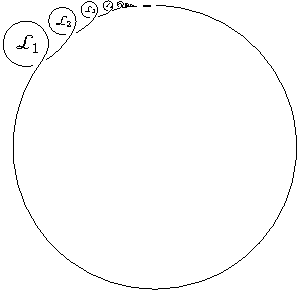
\includegraphics[scale=1]{\figdir/countable-r1.pdf}
  \caption{An unknot that contains countably many crossings.}
\end{figure}
It's not immediately clear that this is something we can \emph{do}
without breaking ambient isotopy, since the result doesn't immediately
appear tame. It turns out that it works, and justifying this is the
first order of business for this chapter.

\section{Countable Reidmeister I
  Moves}\label{sec:countable-r1-moves-for-sn}
In addition to helping us establish connections to permutations, the
theorems in this section will also form the inspiration for our
examination of general topological embeddings in
\cref{part:wild-knots}. The proofs below will not use uniform
convergence (later ones will), and we won't go as deep in
investigating the broader implications of our results so as to avoid
going too far afield.\footnote{The uniform convergence framework is
  more powerful, but it also is \emph{much easier} to accidentally
  misuse. Essentially, it will allow us to drop the ``disjointness''
  conditions in our theorems below, but this will sometimes causes us
  to lose bijectivity on the ambient space and thus break our ambient
  isotopies.} We begin with a straightforward lemma.
\begin{lemma}\label{lem:countable-gluing-homeomorphisms}
  Let $\set{V_n}_{n\in\NN}$ be a collection of closed,
  pairwise-disjoint subsets of $\RR^3$. For all $n \in \NN$, let $f_n
  : \RR^3 \to \RR^3$ be a homeomorphism such that $f_n$ is identity on
  $\RR^3 \setminus V_n^\circ$. Suppose too that%  {\huge \color{red}
    % TRIPLE chec this}
  \[
    \lim_{n\to\infty} \mrm{diam}(V_n) = 0.
  \]
  Then $f$ defined by
  \[
    f(x) =
    \begin{cases}
      f_1(x) & \text{if } x \in V_1 \\
      f_2(x) & \text{if } x \in V_2 \\
      \hspace{.5em} \vdots & \\
      f_n(x) & \text{if } x \in V_n \\
      \hspace{.5em} \vdots & \\
      \hspace{.5em} x & \text{if $x$ is not in any $V_n$}
    \end{cases}
  \]
  is a homeomorphism.
\end{lemma}
\begin{proof}
  First, we show $f$ is a bijection by defining an inverse. Let
  \[
    g(x) =
    \begin{cases}
      f_1^{-1}(x) & \text{if } x \in V_1 \\
      f_2^{-1}(x) & \text{if } x \in V_2 \\
      \hspace{.5em} \vdots & \\
      f_n^{-1}(x) & \text{if } x \in V_n \\
      \hspace{.5em} \vdots & \\
      \hspace{.5em} x & \text{if $x$ is not in any $V_n$}.
    \end{cases}
  \]
  Let $x \in \RR^3$ be arbitrary; we want to show $g(f(x)) = x$. We
  have two simple subcases.
  \begin{enumerate}[label=\arabic*)]
    \item Suppose that for some $n \in \NN$, we have $x \in V_n$. Then
      $g(f(x)) = g(f_n(x)) = f^{-1}_n(f(x)) = x$.
    \item Suppose that there exists no $n \in\NN$ with $x \in V_n$.
      Then $g(f(x)) = g(x) = x$.
  \end{enumerate}
  Hence $g = f^{-1}$, so $f$ is a bijection (as desired).

  Now, we want to show $f$ is continuous. There are any number of ways
  to do this; we choose a more topologically-flavored argument.
  Observe that for all $n \in\NN$, $f\vert_{V_n} = f_n\vert_{V_n}$,
  which is continuous. Hence $f$ is continuous on each $V_n$. One can
  then apply a sequential continuity argument to show $f$ is
  continuous on $X_0 = \ol{\bigcup_{n\in\NN} V_n}$.\footnote{The only
    sneaky case comes in noticing that $x \in X_0$ does not require $x
    \in V_n$ for some $n$. To address it: note that the only other
    case is if $x$ is a limit point of $\bigcup_{n\in\NN}$. Then note
    that because $\mrm{diam}(V_n) \to 0$, one can apply a sequential
    continuity argument to obtain the desired result.
% A quick fix is to notice that $x$ must be a limit
    % point of $\bigcup_{n\in\NN} \partial V_n$, and then apply the fact
    % that $f(x)$ is identity on each $\partial V_n$. Then sequential
    % continuity follows immediately.
  }

  Now observe that $X_q = \RR^3 \setminus \bigcup_{n\in\NN}V_n^\circ$
  is closed, and that $f\vert_{X_1} = \mrm{Identity}\vert_{X_1}$,
  which is continuous. Thus $f$ is continuous on $X_1$. Now, since
  $X_0 \cup X_1 = \RR^3$ and $f$ is continuous on both, the gluing
  lemma gives us that $f$ is continuous on $\RR^3$.

  Applying an identical argument for $f^{-1}$ shows it is continuous
  as well. Hence $f$ is a homeomorphism.
\end{proof}
\begin{remark}
  By taking all but finitely many of the $f_n$ to be identity, we get
  the same result for finite collections of homeomorphisms.
\end{remark}
\begin{remark}
  One can drop the $\mrm{diam}(V_n) \to 0$ condition by assuming the
  collection of $V_n$ is \emph{locally-finite} instead, but this
  precludes us from packing countably-many $V_n$'s into a compact
  space, so we won't use it.
\end{remark}

We have one more elementary lemma before we prove the analogue for
ambient isotopy.
\begin{lemma}\label{lem:endpoints-of-ambient-isotopies-are-embeddings}
  Let $K_0 : [0,1] \times \RR^3 \into \RR^3$, and let $F : [0,1]
  \times \RR^3 \to \RR^3$. Then $K_1 : S^1\into \RR^3$ defined by
  \[
    K_1(s) = F(1, K_0(s))
  \]
  is an embedding.
\end{lemma}
\begin{sproof}
  By definition of an ambient isotopy, $f : \RR^3 \to \RR^3$ defined
  by $f(x) = F(1, x)$ is a homeomorphism. By definition of an
  embedding, $K_0$ is a homeomorphism onto its image, hence $f \circ
  K_0 = K_1$ is too. Thus $K_1$ is an embedding.
\end{sproof}
We now prove our first main result, which is essentially an extension
of \cref{lem:countable-gluing-homeomorphisms} above to ambient
isotopy.
\begin{theorem}[Countable Concatenations of Ambient
  Isotopies]\label{thm:countable-gluing-ambient-isotopies}
  Let $\pn{K_n}_{n\in\NN}$ be a collection of embeddings from
  $S^1\into \RR^3$. Now, suppose that for all $n \in\NN$ there exists
  a closed set $V_n$ such that
  \begin{enumerate}
    \item $K_n \cong K_{n+1}$ by an ambient isotopy $F_n : [0,1]
      \times \RR^3 \to \RR^3$ such that $F_n$ is identity on $[0,1]
      \times (\RR^3 \setminus V_n^\circ)$,
    \item For all $n \neq m$, $V_n \cap V_m = \varnothing$, and
    \item We have
      \[
      \lim_{n\to\infty} \mrm{diam}(V_n) = 0.
      \]
  \end{enumerate}
  Then $K_{\lim} = \lim_{n\to\infty} K_n$ is an embedding, and $K_1
  \cong K_{\lim}$.
\end{theorem}
\begin{proof}
  In light of
  \cref{lem:endpoints-of-ambient-isotopies-are-embeddings}, that
  $K_{\lim}$ is an embedding will follow from our construction of an
  ambient isotopy from $K_0$ to $K_{\lim}$.

  To that end, define $F : [0,1] \times \RR^3 \to \RR^3$ by
  \[
    F(t, x) =
    \begin{cases}
      F_1(t, x) & \text{if } x \in V_1, \\
      F_2(t, x) & \text{if } x \in V_2, \\
      \hspace{1.25em}\vdots & \\
      F_{n-1}(t, x) & \text{if } x \in V_{n-1}, \\
      F_{n}(t, x) & \text{if } x \in V_{n}, \\
      \hspace{1.25em}\vdots & \\
      \hspace{1.125em} x & \text{otherwise.}
    \end{cases}
  \]
  We want to show $F$ is an ambient isotopy.\footnote{To that end,
    recall that we need to show (1) $F(0, x) = x$, (2) For all $s \in
    S^1$, $F(1, K_1(s)) = K_{\lim}(s)$, (3) For all $t \in [0,1]$,
    $F(t, \cdot)$ is a homeomorphism, and (4) $F$ is continuous.}

  Observe that for all $x \in \RR^3$, $F(0, x) = x$, and for all $s
  \in S^1$, $F(1, K_1(s)) = K_{\lim}(s)$ (by construction). Now
  observe that by definition of the an ambient isotopy, for all $t \in
  [0,1]$ and $n \in \NN$, $f_{t,n}(x) = F_n(t, x)$ is a homeomorphism.
  Now, since for all $t \in [0,1]$ we have
  \begin{align*}
    F(t, x) &=
    \begin{cases}
      F_1(t, x) & \text{if } x \in V_1, \\
      F_2(t, x) & \text{if } x \in V_2, \\
      \hspace{1.25em}\vdots & \\
      F_{n-1}(t, x) & \text{if } x \in V_{n-1}, \\
      F_{n}(t, x) & \text{if } x \in V_{n}, \\
      \hspace{1.25em}\vdots & \\
      \hspace{1.125em} x & \text{otherwise}
    \end{cases} \\
    &=
    \begin{cases}
      f_{t,1}(x) & \text{if } x \in V_1, \\
      f_{t,2}(x) & \text{if } x \in V_2, \\
      \hspace{1.25em}\vdots & \\
      f_{t,n-1}(x) & \text{if } x \in V_{n-1}, \\
      f_{t,n}(x) & \text{if } x \in V_{n}, \\
      \hspace{1.25em}\vdots & \\
      \hspace{1.125em} x & \text{otherwise},
    \end{cases}
  \end{align*}
  \cref{lem:countable-gluing-homeomorphisms} implies $F(t, \cdot)$ is
  a homeomorphism. Hence, it just remains to show that $F$ is
  continuous. This follows from the gluing lemma.
  % \begin{itemize}
  %   \item If $(t,x) \in [0,1] \times \RR^3 \setminus
  %     \ol{\bigcup_{n\in\NN} V_n}$, then this follows directly from
  %     $F$ is identity on this set.
  %   \item If $(t,x) \in [0,1] \times V_n^\circ$ for some $n$, this
  %     follows from definition of the $F_n$'s.
  %   \item
  % \end{itemize}

  Note that for all $n \in\NN$, $A_n = [0,1] \times V_n$ is a closed
  set with $F\vert_{A_n}= F_n\vert_{A_n}$. Hence $F$ is continuous on
  $A_n$. Defining $X_0 = \ol{\bigcup_{n\in\NN} A_n}$, we can use a
  similar sequential continuity argument as in
  \cref{lem:countable-gluing-homeomorphisms} to show $F$ is continuous
  on $X_0$.\footnote{Again, the key comes from $\mrm{diam}(V_n) \to 0$
    implying sequential continuity.}

  Similarly, observe that $X_1 = \RR^3 \setminus
  \bigcup_{n\in\NN}V_n^\circ$ is closed, and $F\vert_{X_1} =
  \mrm{Identity}\vert_{X_1}$, hence $F$ is continuous here as well.

  It follows that $F$ is continuous, hence $F$ is an ambient isotopy.
\end{proof}
\begin{proposition}\label{prop:countable-r1-is-valid}
  The countable Reidemeister I move example we described above can be
  realized as the kind of ambient isotopy described in
  \cref{thm:countable-gluing-ambient-isotopies}.
\end{proposition}
\begin{figure}[H]
  \centering
  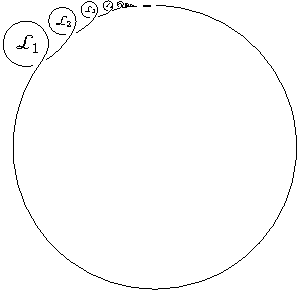
\includegraphics[scale=1]{\figdir/countable-r1.pdf}
  \caption[Countable Reidmeister I Moves]{A countable sequence of
    Reidemeister I moves, for the 3\textsuperscript{rd} time.}
  \label{fig:countable-r1}
\end{figure}
\begin{sproof}[Sketch]
  Without loss of generality, suppose the diagram in
  \cref{fig:countable-r1} represents a projection onto the $xy$ plane.
  Observe that none of the loops in the diagram overlap, so we can
  find closed sets $U_n$ separating each of them when viewed as
  subsets of $\RR^2$. Taking $V_n = U_n \times \RR$ for each $n$, we
  get the desired closed subsets of $\RR^3$. One can then use
  Reidemeister's theorem to argue that we can find ambient isotopies
  $F_n$ representing the process of \np{inserting a single loop in the
    strand in $V_n$ while keeping the boundary fixed}. Applying
  \cref{thm:countable-gluing-ambient-isotopies}, we obtain the desired
  result.
\end{sproof}
\begin{example}
  In a similar manner, one can also employ this result to show that
  cases like the following are possible:
  \begin{figure}[H]
    \centering
    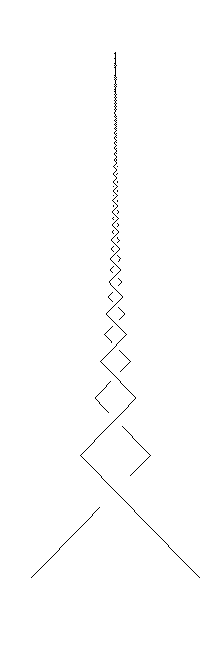
\includegraphics[angle=-90]{\figdir/countable-r2-v2.pdf}
    \caption{Countable Reidemeister II}
    \label{fig:countable-reidemeister-ii}
  \end{figure}
  However, some care is required. Note that it's not immediately
  obvious how we could define the disjoint closed sets $V_n$ --- in
  fact, it seems impossible. The trick is to do it in parts. Suppose
  we start with a caret-shaped arc, like the following:
  \begin{figure}[H]
    \centering
    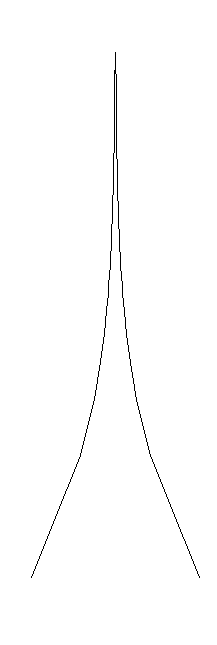
\includegraphics[angle=-90]{\figdir/countable-r2-two-step-0.pdf}
    \caption{A caret-shaped arc}
  \end{figure}
  Insert half of the moves as follows (note, the drawing software
  distorted the figure slightly, so the correspondence with
  \cref{fig:countable-reidemeister-ii} might be a bit hard to see):
  \begin{figure}[H]
    \centering
    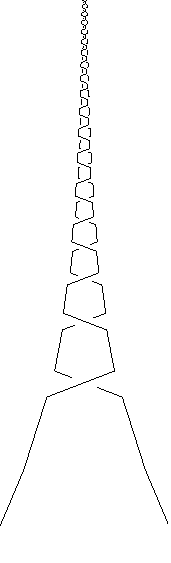
\includegraphics[angle=-90,scale=1.275]{\figdir/countable-r2-two-step-1.pdf}
    \caption{Half of the Reidemeister II moves}
  \end{figure}
  This can be achieved by taking the $V_n$'s to be the dotted regions
  shown in the below.
  \begin{figure}[H]
    \centering
    \hspace{1.5em}
    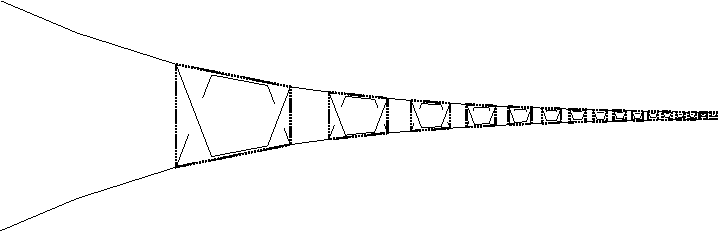
\includegraphics[scale=.9]{\figdir/countable-r2-two-step-1-vs.pdf}
    \caption{The closed neighborhoods, shown with dotted lines}
  \end{figure}
  After this, one can apply a similar technique to the ``flat''
  strands to yield a figure like \cref{fig:countable-reidemeister-ii}.
\end{example}
\begin{remark}
  Although the result might look very similar
  \cref{fig:countable-reidemeister-ii}, to the best of our knowledge,
  the following figure \emph{cannot} be obtained from
  \cref{thm:countable-gluing-ambient-isotopies}.
  \begin{figure}[H]
    \centering
    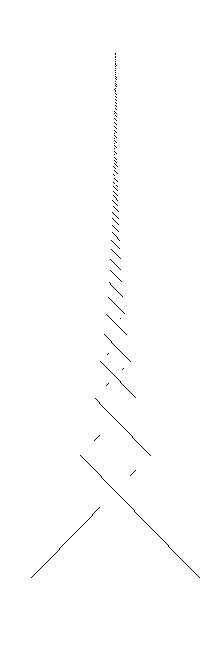
\includegraphics[angle=-90]{\figdir/countable-r1-v2.pdf}
  \end{figure}
  For this, we need the uniform convergence form of
  \cref{thm:countable-gluing-ambient-isotopies}, which we prove in
  \cref{thm:uniformly-convergent-ambient-isotopy}.
  % {\color{blue} HYPERLINK THIS}
\end{remark}

\subsection{An Alternative Argument:
  A $C^1$ Parameterization}\label{sec:c1-countable-r1}
In case the arguments above are not convincing, we have constructed an
explicit parameterization of an arc with a diagram similar to that of
\cref{fig:countable-r1} that is $C^1$ embedded in
$\RR^3$.\footnote{This is proven in \cite{Crowell1963} to be
  sufficient to guarantee tameness --- see \cref{chap:feral-gallery}
  for more details, as well as some other examples.} The idea behind
the parameterization is as follows: take a big circle and a small
circle, where the center of the small circle lies on the circumference
of the big circle, and the plane of the small circle is normal to the
tangent vector of the big circle. Let $\theta$ denote the polar angle
of the big circle, and $r$ its radius. As $\theta \to 0$, we'll make
the radius of the small circle decay like $r\theta^3$, while watching
a point on its circumference oscillate with frequency $\propto
\frac{\omega}{\theta}$. $C^1$-ness will then follow from the
$C^1$-ness of the function
\begin{equation}\label{eq:g-equation}
  g(\theta) =
  \begin{cases}
    r\theta^3 \sin\pn{\frac{\omega}{\theta}} & \theta \neq 0 \\
    0 & \theta = 0
  \end{cases}
\end{equation}
for $r, \omega > 0$.
\begin{proposition}
  Consider $f : [0, \pi/3] \to \RR^3$ defined\footnote{We choose the
    domain $[0, \pi/3]$ just because it looks nice with the rest of
    the parameters we chose when plotting. This quirk can be removed
    by inserting constants in various places.} by: $f(0) = 0$, and for
  all $\theta \in (0, \pi/3]$,
  \begin{align*}
    f(\theta) &=
                \underbrace{
    \begin{bmatrix}
      0 & \frac{\cos(\theta)}{r} & 0 \\
      0 & \frac{\sin(\theta)}{r} & 0 \\
      1 & 0 & 0
    \end{bmatrix}}_{M}
              \underbrace{
    \begin{bmatrix}
      \theta^3\sin\pn{\frac{\omega}{\theta}} \\
      \theta^3\cos\pn{\frac{\omega}{\theta}} \\
      0
    \end{bmatrix}}_{\bm v} +
    \underbrace{
    \begin{bmatrix}
      r \cos(\theta) \\
      r \sin(\theta) \\
      0
    \end{bmatrix}}_{\mb v_0} \\
    &=
      \begin{bmatrix}
        \frac{t^3 \cos(t) \cos(\omega/t)}{r} + r\cos(\theta) \\
        \frac{t^3 \cos(t) \sin(\omega/t)}{r} + r\sin(\theta) \\
        t^3 \sin(\omega/t)
      \end{bmatrix}
  \end{align*}
  Then $f$ is $C^1$ on $(0,\pi/3)$, and $\lim_{\theta\to 0^+}
  f'(\theta) = (0,r,0)$.\footnote{In fact $\lim_{\theta \to 0}
    f'(\theta) = (0,r,0)$ as well (not just from the $0^+$ side), we
    just included right-handed limit to emphasize that we've only
    defined $f$ on $[0,\pi/3]$. On that note, $\lim_{\theta\to
      \pi/3^-} f'(\theta)$ exists as well, but that's not really a
    surprise --- the only place things could really go wrong are at
    $\theta = 0$.}
\end{proposition}
\begin{remark}
  In the equations above, $M$ rotates us into the orthogonal frame for
  the big circle's tangent vector (here, the big circle is
  parameterized to lie in the $xy$-plane), $\mb v$ represents the
  point on the circumference of the small circle, and $\mb v_0$ shifts
  the result so that the center of the small circle would lie on the
  circumference of the big circle.
\end{remark}
\begin{sproof}
  One can argue that $\lim_{\theta \to 0} f'(\theta)$ exists by noting
  that the function $g(\theta)$ defined in \cref{eq:g-equation} is
  $C^1$, and then using the product rule, etc. Feeding it into
  \texttt{Mathematica} also works.

  It follows that $f(\theta)$ can be extended to a $C^1$ function $f :
  S^1 \into \RR^3$.
\end{sproof}
We now provide some plots. Code for an interactive 3D version using
\texttt{Julia} can be found in
\cref{sec:Julia-for-countable-reidemeister-i}
\begin{figure}[H]
  \centering
  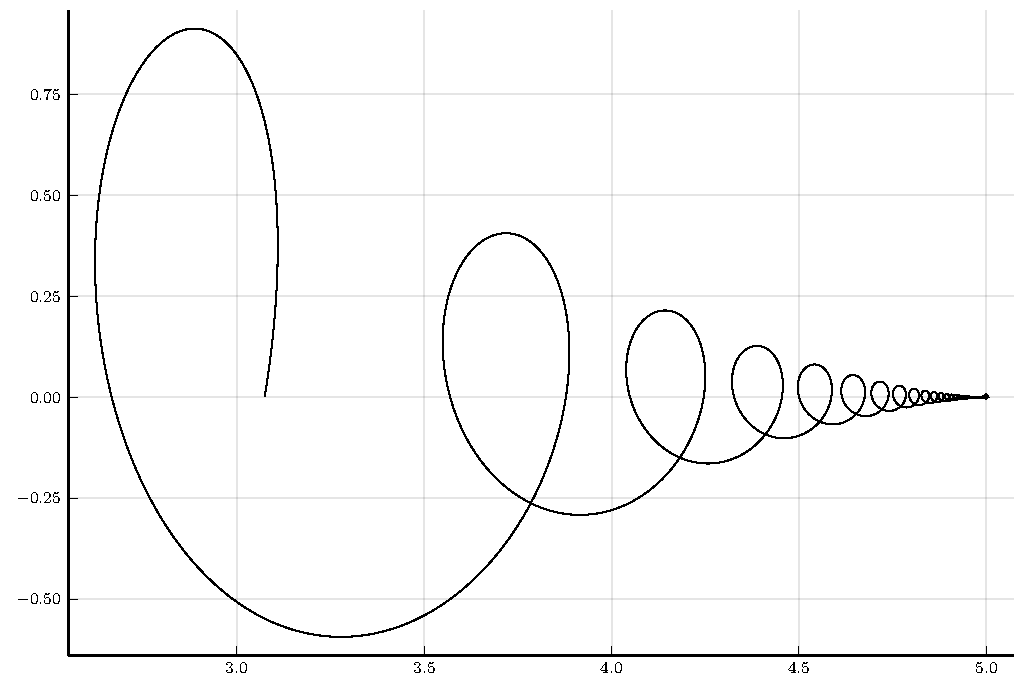
\includegraphics[scale=.5]{\figdir/smooth-countable-3d-spiral.pdf}
  \caption[Parameterized countable Reidemeister I]{The parameterized
    function with $r=5$, $\omega=2\pi^2$, here projected onto the $xz$
    plane.}
\end{figure}
\begin{figure}[H]
  \centering
  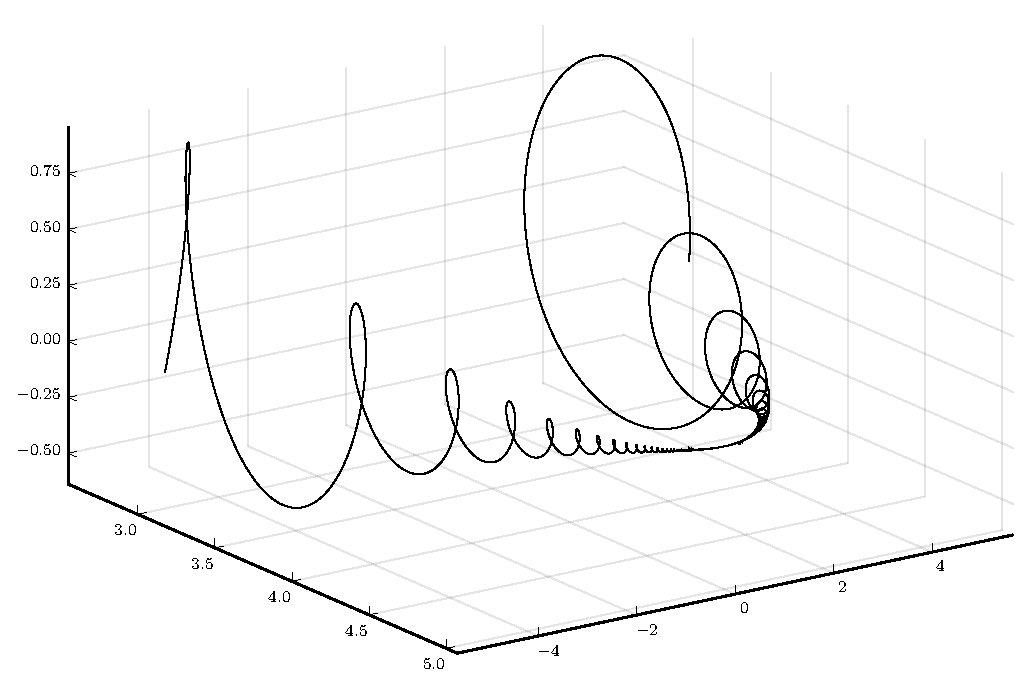
\includegraphics[scale=.5]{\figdir/smooth-countable-3d-spiral-in-3d.pdf}
  \caption[A 3D view]{A $3$D view of a version defined over $[-\pi/3,
    \pi/3]$.}
  \label{fig:3d-countable-reidemeister-i-plot}
\end{figure}
Note, if we were to use $\theta^2$ instead of $\theta^3$, we'd lose
the $C^1$ condition, but it'd still yield some pretty plots.
\begin{figure}[H]
  \centering
  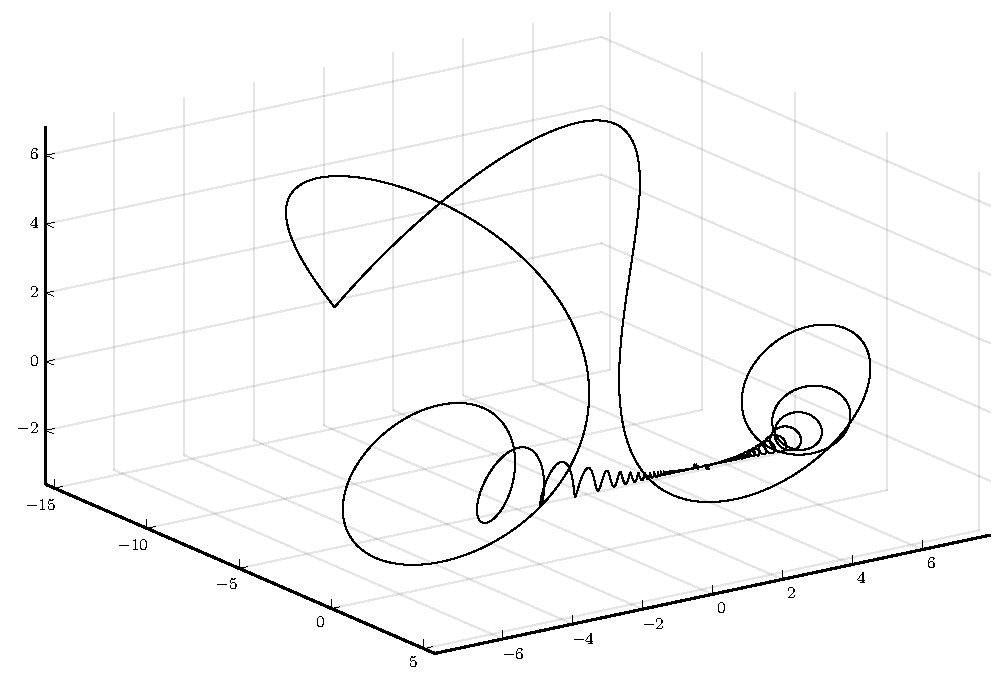
\includegraphics[scale=.75]{\figdir/countable-3d-spiral.pdf}
  \caption{Using $\theta^2$ instead}
\end{figure}
So, to recap: we've shown that under certain mild conditions, we can
apply countably-many Reidemeister moves to our knots and still yield
tame embeddings. We use this to create our desired representation in
terms of $S_n$.
%  We use this for a brief venture into trying to
% connect Gauss codes to the finitary symmetric group.


\section{Using Countable-Crossings to Define an
  Action}\label{sec:defining-the-action}
The effects of the \cref{prop:countable-r1-is-valid} can be summarized
as ``we can create many bounded, tame arcs that have infinitely many
crossings.'' We apply this to create our combinatorial representation.
Note that in our creation of a ``standard unknot code,'' we're
imagining a slightly modified version of
\cref{prop:countable-r1-is-valid} in which we insert \emph{both} a $+$
and a $-$ version of crossing $k$ using Reidemeister I moves. While it
might seem strange to have \emph{two} crossings labeled by $k$ in our
Gauss codes, this will turn out to be more natural for our purposes.
Further, we'll see that only one can appear nontrivially (i.e., not
locally removable by a Reidemeister I move) at any given time.

In deciding how to add both of these $+$/$-$ characters, we've elected
to define the standard unknot in a way that the process corresponds to
the insertion of a framed Reidemeister I move for each $k$.
\begin{definition}[Standard Gauss sequence for the unknot]
  The \emph{standard Gauss sequence for the unknot}, denoted $コ_\maru$,
  is defined by
  \begin{align*}
    コ_\maru
    &= \csum_{k = 1}^\infty (k_u^+, k_o^+, k_o^-, k_u^-) \\
    &= {1_u^+, 1_o^+, 1_o^-, 1_u^-, 2_u^+, 2_o^+, 2_o^-, 2_u^-,
      \ldots, n_u^+, n_o^+, n_o^-, n_u^-, \ldots} \qedhere
  \end{align*}
\end{definition}
\begin{figure}[H]
  \centering
  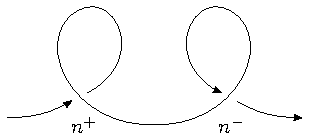
\includegraphics{\figdir/framed-r1-labeled.pdf}
  \caption[One of the blocks]{An example of one of the inserted blocks}
\end{figure}
\begin{question}
  Is this the most natural choice of canonical representative for
  $\maru$? After reading the below and seeing the way we try and use
  $コ_\maru$ in our Symmetric group formalism, the reader is
  encouraged to ponder this question. The author would be excited to
  hear any insights!
\end{question}
We use this to define the standard Gauss sequence for a knot $K$ in a
way that will be germane to viewing it in terms of permutations. The
idea is very simple (we're basically just inserting the symbols that
are missing from $コ_\maru$ in $コ_K$ in the places they would be in
$コ_\maru$), but the notation in the below is almost laughably
verbose. This is because we were trying to define things as precisely
as possible to make translation into computer programs easier. We
encourage the reader to reference the examples if the definition is
hard to parse.
\begin{definition}[Standard Gauss Sequence]\label{prop:infinite-gauss-sequence}
  Let $K$ be an $n$-crossing knot given by some signed Gauss code $コ_K
  = k_{1,x_1}^{\epsilon_1}, k_{2, x_2}^{\epsilon_2}, \ldots, k_{2n,
    x_{2n}}^{\epsilon_{2n}}$. Note, in $コ_K$ we have indexed
  $\epsilon_i$ by $i = 1, \ldots, 2n$ to describe the sign of the
  \np{crossing partially represented by the $i$\textsuperscript{th}
    symbol in $K$}.\footnote{``Partially'' because each crossing is
    encoded by two symbols in $コ_K$} We'll define a related set of
  symbols (here labeled as $\neg \mu_j$ over $j = 1, \ldots, n$) by
  ``$\neg \mu_j$ is the \emph{opposite} of the sign of crossing $j$ in
  $K$.'' Again, to be extra clear, note the difference in indexing ---
  $i$\textsuperscript{th} symbol, $j$\textsuperscript{th} crossing.
  The symbol $\mu$ is chosen just to avoid confusion with the
  $\epsilon$'s; the $\neg$ is to emphasize the fact that we want the
  opposite of the sign of crossing $k$.

  We'll also define symbols $\alpha_j, \beta_j$ by
  \begin{itemize}
    \item If $\neg \mu_j = -$, then $\alpha_j = o$, $\beta_j = u$.
    \item If $\neg \mu_j = +$, then $\alpha_j = u$, $\beta_j = o$.
  \end{itemize}
  Use these to construct a sequence of $n$ 4-symbol blocks $b_j$ as
  follows:
  \begin{itemize}
    \item If $\neg \mu_j = -$, then $b_j$ is given by
      \[
      b_j = k_{2j-1,x_{2j-1}}^{\epsilon_{2j-1}} k_{2j,
      x_{2j}}^{\epsilon_{2j}} j_{\alpha_j}^{\neg \mu_j}
      j_{\beta_j}^{\neg \mu_j},
      \]
      and
    \item If $\neg \mu_j = +$, then $b_j$ is defined by
      \[
      b_j = j_{\alpha_j}^{\neg \mu_j} j_{\beta_j}^{\neg \mu_j}
      k_{2j-1,x_{2j-1}}^{\epsilon_{2j-1}} k_{2j,
      x_{2j}}^{\epsilon_{2j}}.
      \]
  \end{itemize}
  Then we overwrite the definition of $コ_K$ to be a string of $4n$
  symbols constructed by concatenating the $b_j$,
  \[
    コ_K^{\rm fin} = \csum_{j=1}^n b_j.
  \]
  We call this the \emph{finite portion} of the \emph{standard Gauss
    sequence representation}. The full \emph{standard Gauss sequence
    representation} is given by
  \[
    コ_K = コ_K^{\rm fin} \csum \pn{\csum_{k=2n+1}^\infty k_u^+,
      k_o^+, k_o^-, k_u^-}. \qedhere
  \]
\end{definition}
From now on, when we write $コ_K$, unless otherwise stated, we are
thinking of the standard Gauss sequence representation. The following
proposition asserts that $コ_K$ is realizable by ambient isotopy (up
to relabeling to ensure both the $+$ and $-$ copies of crossing $k$
are included).
\begin{proposition}
  Let $K$ be an $n$-crossing knot. Then the underlying geometric
  representative for $K$ is ambient isotopic to one realizing the
  standard Gauss sequence for $K$ (with some minor relabeling to
  ensure both $k^+$, $k^-$ appear).
\end{proposition}
\begin{sproof}
  Immediate from the construction of $コ_K$. Insert the finitely-many
  Reidemeister I moves as dictated by the $j^{\neg \mu_j}_{\alpha_j}$,
  $j^{\neg \mu_j}_{\beta_j}$ to construct $コ_K^{\rm fin}$, and then
  apply \cref{thm:countable-gluing-ambient-isotopies} to yield the
  infinite tail.
\end{sproof}
We now provide some examples of the $コ_K^{\rm fin}$, and show how
they compare to equivalent-length standard unknot sequences.
\begin{note}
  \textbf{IMPORTANT!} We \emph{highly} recommend the reader try
  interacting with some of the concepts below programmatically. If
  desired, \href{https://www.sagemath.org/}{\texttt{sage}}\footnote{If
    the link doesn't work: \url{https://www.sagemath.org/}} code can
  be found open-source
  \href{https://github.com/redpanda1234/permutation-knots}{here}\footnote{If
    the link doesn't work:
    \url{https://github.com/redpanda1234/permutation-knots}} on
  Github.

  At the time of writing, the code is mainly in the prototyping phase,
  hence documentation is not extensive, and we have not done thorough
  bug-testing. However, basic functionality appears to be quite solid.
  If the reader has any questions and/or encounters a bug, we heavily
  encourage them to submit an
  \href{https://github.com/redpanda1234/permutation-knots/issues}{issue
    report}\footnote{If the link doesn't work:
    \url{https://github.com/redpanda1234/permutation-knots/issues}},
  or to contact the author at \texttt{fkobayashi@g.hmc.edu}.
\end{note}
\begin{example}[Standard Gauss Sequences]\label{ex:standard-gauss-sequences}
  In the following, we'll highlight the newly-inserted portions gray.
  \begin{itemize}
    \item Consider the trefoil given by $1^+_u, 2^+_o, 3^+_u, 1^+_o,
      2^+_u, 3^+_o$. Then $コ_{(3,1)}^{\rm fin}$ is given by
      \[
      コ_{(3,1)}^{\rm fin} = 1^+_u, 2^+_o, {\color{gray} 1^-_o,
      1^-_u}, 3^+_u, 1^+_o, {\color{gray} 2^-_o, 2^-_u}, 2^+_u, 3^+_o,
      {\color{gray} 3^-_o, 3^-_u}.
      \]
      Compare this to the finite part of the standard unknot sequence
      of the same length. We've grayed out the same portions in the $
      コ_\maru$ as in $コ_{(3,1)}^{\rm fin}$ to focus the reader's
      eyes on the differences.
      \begin{align*}
        コ_\maru
        &= 1^+_u, 1^+_o, {\color{gray} 1^-_o, 1^-_u}, 2^+_u, 2^+_o,
          {\color{gray} 2^-_o, 2^-_u}, 3^+_u, 3^+_o,
          {\color{gray}3^-_o, 3^-_u} \\
        コ_{(3,1)}^{\rm fin}
        &= 1^+_u, 2^+_o, {\color{gray} 1^-_o, 1^-_u}, 3^+_u, 1^+_o,
          {\color{gray} 2^-_o, 2^-_u}, 2^+_u, 3^+_o, {\color{gray}
          3^-_o, 3^-_u}
      \end{align*}
    \item The purpose of the definition of the $b_j$'s is more
      apparent in knots where not every crossing is the same sign.
      Consider the figure eight knot given by Gauss code $1^-_u,
      2^-_o, 3^+_u, 4^+_o, 2^-_u, 1^-_o, 4^+_u, 3^+_o$. Then compare $
      コ_\maru$ and $コ_{(4,1)}^{\rm fin}$:
      \begin{align*}
        コ_\maru
        &=
          {\color{gray}1^+_u 1^+_o}, 1^-_o 1^-_u, {\color{gray} 2^+_u
          2^+_o}, 2^-_o 2^-_u, 3^+_u 3^+_o, {\color{gray} 3^-_o 3^-_u},
          4^+_u 4^+_o, {\color{gray} 4^-_o 4^-_u} \\
        コ_{(4,1)}^{\rm fin}
        &=
          {\color{gray}1^+_u 1^+_o}, 1^-_u 2^-_o, {\color{gray} 2^+_u
          2^+_o}, 3^+_u 4^+_o, 2^-_u 1^-_o, {\color{gray} 3^-_o 3^-_u},
          4^+_u 3^+_o, {\color{gray} 4^-_o 4^-_u}
      \end{align*}
    \item Finally, we give the example of the $(6,1)$ knot given by
      \[
      1^+_u, 2^+_o, 3^-_u, 4^-_o, 5^-_u, 6^-_o, 2^+_u, 1^+_o, 6^-_u,
      5^-_o, 4^-_u, 3^-_o.
      \]
      The codes are {\scriptsize
      \begin{align*}
        コ_\maru
        &= 1^+_u 1^+_o, {\color{gray} 1^-_o 1^-_u}, 2^+_u 2^+_o,
          {\color{gray} 2^-_o 2^-_u, 3^+_u 3^+_o}, 3^-_o 3^-_u,
          {\color{gray} 4^+_u 4^+_o}, 4^-_o 4^-_u, {\color{gray} 5^+_u
          5^+_o}, 5^-_o 5^-_u, {\color{gray} 6^+_u 6^+_o}, 6^-_o
          6^-_u\\
        コ_{(6,1)}^{\rm fin}
        &= 1^+_u 2^+_o, {\color{gray} 1^-_o 1^-_u}, 3^-_u 4^-_o,
          {\color{gray} 2^-_o 2^-_u, 3^+_u 3^+_o}, 5^-_u 6^-_o,
          {\color{gray} 4^+_u 4^+_o}, 2^+_u 1^+_o, {\color{gray} 5^+_u
          5^+_o}, 6^-_u 5^-_o, {\color{gray} 6^+_u 6^+_o}, 4^-_u
          3^-_o
      \end{align*}} \qedhere
  \end{itemize}
\end{example}
\noindent The point of the above is that we can think of signed Gauss
codes as infinite sequences where finitely many of the terms have been
derranged. Using this, we can begin to formally establish connections
between knot equivalence and the finitary symmetric group on a
countable set. Recall the following:
\begin{definition}[Group Action]
  Let $(G, \cdot)$ be a group with identity element $e$, and let $S$
  be a set. Let $\varphi : G \times S \to S$ such that for all $s \in
  S$,
  \begin{enumerate}
    \item $\varphi(e, s) = s$, and
    \item For all $g,h \in G$,
      \[
      \varphi(g \cdot h, e) = \varphi\pn{g, \varphi\pn{h, e}} \qedhere
      \]
  \end{enumerate}
\end{definition}
% The \emph{Finitary Symmetric Group} is the group of all permutations
% on $\NN$ that fix all but finitely many elements.
\begin{definition}[Finitary Symmetric Group]
  Let $\ms N$ be a countable set. Then the set $S_{\aleph_0}$ of all
  bijections $f : \ms N \to \ms N$ forms a group under function
  composition. Consider the subgroup $S_{\rm fin}$ defined by
  \[
    S_{\rm fin} = \set{\sigma \in S_{\aleph_0} \MID \sigma \text{
        fixes all but finitely many } n \in \ms N}.
  \]
  We call $S_{\rm fin}$ the \emph{finitary symmetric group} on $\ms
  N$.
\end{definition}
Given the definitions above, we'll usually think about $\ms N$ as
being a collection of the characters
\[
  \ms N = \bigcup_{k \in \NN} \set[]{k_u^+, k_o^+, k_o^-, k_u^-},
\]
in which case we denote $\ms N$ by $\ms N_{\rm str}$. However, we'll
note that there's another interesting set of characters we can use
that yields some nice properties.
\begin{definition}[$\ZZ{[i]}$ Representation of Gauss sequences]
  For the sake of notational compactness, let $\ms N_{\text{g.int}} =
  \ZZ \cup i\ZZ$ (i.e., the set of all purely real or purely imaginary
  elements of $\ZZ[i]$).\footnote{``g. int'' is used to suggest
    ``Gaussian integers.''} Define a bijection $f : \ms N_{\rm str}
  \to \ms N_{\text{g.int}}$ by
  \begin{align*}
    f(k_u^+)
    &= -k
    &
      f(k_u^-)
    &= -k \cdot i \\
    f(k_o^+)
    &= k
    &
      f(k_o^-)
    &= k\cdot i
  \end{align*}
  observe that $f$ is indeed a valid bijection. Hence, using $\ms
  N_{\rm g.int}$ as our set of label characters is fully equivalent to
  using $\ms N_{\rm str}$.
\end{definition}
Observe that multiplying $コ_K^{\rm fin}$ by $i$ gives the obverse,
while multiplying by $i^2 = -1$ gives the reverse.

Independent of whichever set we choose to be our alphabet for forming
the Gauss code strings, we have the following proposition.
\begin{proposition}\label{prop:knots-as-permutations}
  For each knot $K$ represented by a \emph{standard} signed Gauss
  sequence $コ_K$, $コ_K$ can be realized as the action of an element
  $\sigma_K \in S_{\rm fin}$ on the standard signed Gauss sequence for
  the unknot, $コ_\maru$.
\end{proposition}
\begin{sproof}
  By construction of the standard Gauss sequence, writing the $コ_\maru$
  and $コ_K$ on two adjacent lines, one can immediately see the
  correspondence with the two-line notation for $\sigma_K$:
  \[
    コ_{\maru} \xmapsto{
      \begin{pmatrix}
        1^+_u & 1^+_o & 1^-_o & \cdots & n^-_u \\
        \sigma_K(1^+_u) & \sigma_K(1^+_o) & \sigma_K(1^-_o) & \cdots &
        \sigma_K(n^-_u)
      \end{pmatrix}
    } コ_K.
  \]
  Note that exactly one of the pairs $(1^+_u, 1^+_o)$, $(1^-_o,
  1^-_u)$ is fixed by $\sigma_K$.
\end{sproof}
From this, we can calculate the cycle representation of our
permutations. Full tables for the cycle representation of knots up to
$8$ crossings are given in \cref{app:combinatorial-representations} in
\cref{tab:cycle-gint} (using the $\ms N_{\rm g.int}$ notation) and in
\cref{tab:cycle-str} (using the $\ms N_{\rm str}$ representation).
Again, the code we used to work with these can be found on
\href{https://github.com/redpanda1234/permutation-knots}{Github}.\footnote{Once
  more, if the link doesn't work:
  \url{https://github.com/redpanda1234/permutation-knots}}.

\subsection{The Problem with Equivalence}
Interpreting \emph{knot equivalence} in this context gets a bit
thorny, and it seems that there's likely no way to make it compatible
with the group structure (although we have not explicitly constructed
counterexamples). On the one hand, viewed in abstraction, the
Reidemeister moves can clearly be defined in terms of elements $\sigma
\in S_{\rm fin}$, as detailed by the following proposition.
\begin{proposition}
  Let $の$, $ゆ$, and $め$ denote the Reidemeister I, II, and III
  moves, respectively.\footnote{These characters are Hiragana
    \emph{no} (\ipa{no}), \emph{yu} (\ipa{jW}), and \emph{me}
    (\ipa{め}). We choose them for their visual similarity to
    diagrammatic representations of our Reidemeister moves.} Then the
  collections of all valid $の$, $ゆ$ and $め$ moves (denoted $S_{の}$,
  $S_{ゆ}$, and $S_{め}$) form countable subsets of $S_{\rm fin}$.
\end{proposition}
\begin{sproof}
  We just consider the case of $の$; the others are identical. Let
  $K_0, K_1$ be knots with Gauss sequences $コ_{K_0}$, $コ_{K_1}$,
  such that $K_0$ is related to $K_1$ by applying a single
  Reidemeister move. By \cref{prop:knots-as-permutations}, we can
  represent them by permutations $\sigma_{K_0}$, $\sigma_{K_1} \in
  S_{\rm fin}$ such that
  \[
    コ_{K_0} = \sigma_{K_0} \cdot コ_\maru
    \qquad\text{and}\qquad コ_{K_1} = \sigma_{K_1}\cdot コ_\maru.
  \]
  Hence
  \begin{align*}
    \sigma_{K_0}^{-1} \cdot コ_{K_0}
    &= コ_\maru \\
    &= \sigma_{K_1}^{-1} \cdot コ_{K_1},
  \end{align*}
  and thus we have
  \[
    \sigma_{K_1} \sigma_{K_0}^{-1} コ_{K_0} = コ_{K_1}.
  \]
  Then define $\sigma_{の, K_0 \to K_1}$ by
  \[
    \sigma_{の, K_0 \to K_1} = \sigma_{K_1} \sigma_{K_0}^{-1},
  \]
  and observe that it is an element of $S_{\rm fin}$ realizing the
  desired $の$ move. By considering all such $K_0$, $K_1$, we can show
  that we get countably many such $\sigma$ that act nontrivially on
  the unknot in distinct ways, which proves the claim.
\end{sproof}
On the other hand, it's worth noting that applying $\sigma_{の, K_0
  \to K_1}$ to the Gauss sequence for some other knot $K_2$ might not
yield a $の$-type move, and similarly with $ゆ$ and $め$. In fact,
it's unclear whether fully unrestricted use of such moves might allow
for arbitrary permutations of the Gauss codes, and thus unknotting
operations. We summarize this in the following question:
\begin{question}
  Is $\ip{S_の} = \ip{S_ゆ} = \ip{S_め} = S_{\rm fin}$? Since it
  suffices to check whether or not each of the moves can be used to
  define arbitrary transpositions, this seems straightforward to
  check, but we haven't had time to examine it yet. It's worth noting
  that one should be extra careful to note that the definition of the
  Gauss code Reidemeister moves is encoded in terms of one-line
  notation, \emph{not} cycle notation.

  If the equality does not hold for at least one of the moves (suppose
  it's $S_の$), then we get a subgroup. What does it look like? What
  do the cosets look like? To what extent do they correspond with
  equivalence classes of diagrams under Reidemeister I?
\end{question}
This is symptomatic of the bigger problem with trying to use $S_{\rm
  fin}$ to discuss knot equivalence: Essentially, no matter what we
do, determining which $\sigma \in S_{\rm fin}$ we're allowed to apply
to a knot $K$ seems to require specific knowledge about $K$ itself.
Here are some descriptions of why. In all of the following, let $K$ be
an $n$-crossing knot with Gauss sequence $コ_K$.
\begin{itemize}
  \item Say we want to perform a Reidemeister I move between crossings
    $i$ and $j$. This can be accomplished by a $\sigma_の$ move that
    essentially shifts the entire portion of $コ_K$ from $j$ onwards to
    the right, while moving the corresponding
    $(n+1_{x_n+1}^{\epsilon_{n+1}}, n+1_{\neg x_n+1}^{\neg
    \epsilon_{n+1}})$ block to appear right after $i$, and then
    relabeling the $n+1 - j$ crossings we've just modified so that
    they're in increasing order once again. The problem here is that
    if we try and apply this move to another knot, say one with $m >
    n$ crossings. Suddenly, it's not clear that the permutations we
    used to define the above can be used, since the
    $n+1$\textsuperscript{st} crossing might be involved in a
    nontrivial portion of the knot.

  \item Reidemeister II suffers from similar concerns.
  \item For Reidemeister III, the permutations $\sigma_め$ employed
    are comparatively simple to define, but we have to be careful
    about when exactly we can use them. In particular, the constraint
    that we have to start with a Gauss code of a certain form in order
    to apply the move is troubling.
  \item Even removing the dependence on the choice of basepoint seems
    nontrivial, since this would require permuting \emph{only} the
    portions of $コ_K^{\rm fin}$ that did not arise from the
    $j_{\alpha_j}^{\neg mu_j}$, $j_{\beta_j}^{\neg \mu_j}$. Again,
    this would require specific knowledge of $K$.
\end{itemize}
There are a number of possible directions for future work that could
address these issues.
\begin{enumerate}
  \item Can we find a way to interpret the signed Gauss sequence in a
    way that's more labeling-agnostic? For instance, if we were to
    insert a countable number of ``blank'' characters between each of
    the non-trivial symbols in $コ_K$ (i.e., the non
    $j_{\alpha_j}^{\neg \mu_j}$, etc. ones), then we could resolve the
    problem of Reidmeister I and Reidmeister II by just thinking about
    exchanging the labels for the new crossings we're inserting with
    an appropriate choice of blank characters.

    One way to achieve something like this would be to think
    of $コ_\maru$ as actually representing all of $\QQ$, together with
    appropriate $+$/$-$ and $u$/$o$ symbols. Then, if we want to
    insert a crossing between crossings $1$ and crossing $2$, instead
    of doing the shifting and relabeling process we described for
    Reidemeister I, we could think the operation as inserting a
    crossing $\frac{1}{2}$. Of course, this would require us to create
    a knot that has a crossing everywhere on an embedded copy of $\QQ$
    in $S^1$, which it seems we can do using
    \cref{thm:uniformly-convergent-ambient-isotopy}. % {\color{blue} using the uniform
    % convergence formalism later.
    The particular construction we'd use solves the problem of
    Reidmeister I, but still leaves the issues of Reidemeister II and
    Reidemeister III. We wonder whether using this, there's a way to
    construct a standard unknot that is ``universal'' for Reidmeister
    I \emph{and} II moves simultaneously, in the sense that our
    $コ_\maru$ is for Reidemeister I.
  % \item Another direction for possible work is to see \emph{if} \np{in
  %   writing down the messy equivalence relation described in the
  %   bulleted section above} there's any way we can find a simpler
  %   generating set for the equivalence relation. This seems quite
  %   unlikely, but we won't rule it out.
  % \item A final possibility is that clean group-like structure is
  %   simply too much to ask for
  \item Even if it turns out Reidemeister equivalence is just too much
    to ask for from a group-like structure, it seems that the
    formalism described above certainly yields a nice framework for
    categorification of knots. For instance, one could create a
    subcategory for \np{each Reidemeister equivalence class of knots}
    in which the objects are sequences in one of the $\ms N$, and the
    morphisms are the $\sigma \in S_{\rm fin}$ that correspond to
    valid Reidmeister moves. In this context, we could view
    \emph{unknotting operations} in terms between these subcategories.
    We'd be interested to see if interesting structure can arise out
    of this perspective.
\end{enumerate}
The point is that equivalence seems challenging to incorporate,
especially given the difficulty in working with the formalism above
without some guiding conjectures. Hence, we leave this as a direction
for future work, and shift instead to summarizing some of our
computational results.

%  collect some computational results in the
% meantime.

% and
% we have not yet had an opportunity to push our questions here as far
% as we would like.

% As
% working with the formalism by hand can be unpleasant without guiding
% conjectures, we believe computational approaches hold the most
% promise. We describe some preliminary work on this in the below,
% together with a large collection of directions for future work.

% Owing to time constraints, work was spent trying to work out exactly
% what was going on with wild vs.\ tame knots so that we could employ
% the example of countable sequences of Reidemeister I moves to generate
% the formalism. Hence, in lieu of a grand collection of theorems, we'll
% just list some computational observations and then give a list of
% future projects we'd be interested in pursuing. Of course, we
% encourage the reader to take a crack at anything that sounds
% interesting.

\section{Computational Observations \& Directions for Future
  Work}\label{sec:computational-observations-and-future-work}
As we've stated twice before, source code for the following can be
found on \href{https://github.com/redpanda1234/permutation-knots}{Github}.\footnote{
  \url{https://github.com/redpanda1234/permutation-knots}}.

Based on our \texttt{sage} computations, we've noticed the following
patterns.\footnote{Note, whenever we say ``up to $8$ crossings,'' that
  does not mean the bound is sharp; rather, it is just that we have
  not tried higher crossing-number knots.}
\begin{itemize}
  \item For any two knots $K_0$, $K_1$ with up to $8$ crossings, when
    the products $\sigma_{K_0} \sigma_{K_1}$ and $\sigma_{K_1}
    \sigma_{K_0}$ act on $コ_\maru$, it appears that (after
    relabeling) the result is a prime knot.\footnote{We should note
    that our primality checker was not terribly sophisticated, hence
    there could be a flaw in it. Essentially, the program just
    recursively removed all possible Reidemeister I and Reidemeister
    II moves and then checked the result for an obvious point to cut
    the Gauss code.} We would like to see if this can be verified
    theoretically, and if not, whether it still tends to hold ``most''
    of the time as $n \to\infty$. This seems very unlikely to us, but
    we'd be willing to be surprised.
  \item For classical knots $K_0$, $K_1$, it is possible for
    $\sigma_{K_0} \sigma_{K_1}$ to act on $コ_\maru$ to yield a
    virtual knot. For example, $(\sigma_{(6,3)} \sigma_{(6,2)}) \cdot
    コ_\maru$ yields a virtual trefoil with code $4^-_o, 6^+_o, 4^-_u,
    6^+_u$. By contrast, $(\sigma_{(6,2)}\sigma_{(6,3)}) \cdot コ_\maru$
  \item We computed the length of the Reidemeister I / II reduced
    forms of the Gauss codes resulting from all pairwise
    multiplications up to $8$ crossings (see \cref{tab:mult-table} for
    explicit numbers, and \cref{tab:mult-heatmap} for a heatmap). In
    general, it seems the heatmap is approximately symmetric. We
    wonder whether this can be explained purely in terms of the
    permutations.
  \item We have also made a log-scale plot of the orders of the groups
    that are generated pairs of the $\sigma_{K}$ (see
    \cref{tab:po-heatmap}). We wonder whether there's any correlation
    with \cref{tab:mult-heatmap}. We'd also be curious to see whether
    the patches that appear have interpretable meaning.
\end{itemize}
We'd be interested in seeing further work in understanding these
observations. In addition to the above, we have the following
questions for further work:
\begin{itemize}
  \item How do we interpret the multiplication operation in $S_{\rm
    fin}$ topologically? One hiccup is that if crossing $k$ appears
    with two different signs in $\sigma_{K_0}$, $\sigma_{K_1}$, then
    we have to relabel in the product to interpret the result. But
    putting that aside, the primality phenomenon described above seems
    very intriguing, and we would like to see diagrammatic
    interpretations of what's going on.
  \item We can represent the $\sigma_K$ by permutation matrices that
    have been padded with countable sequences of $0$'s. As $n \to
    \infty$, how are the non-zero parts of these matrices distributed
    in the space of $n\times n$ matrices?
  \item We described earlier how we can think of Reidemeister moves as
    describing subsets of $S_{\rm fin}$. We reiterate the questions we
    had then: Do these subsets generate $S_{\rm fin}$ in full? If not,
    they form subgroups; what do the cosets look like? So on and so
    forth.
\end{itemize}


% We now state some propositions describing how we can think of
% combinatorial equivalence of Gauss codes in terms of this formalism.
% \begin{proposition}
%   Let
% \end{proposition}



% However, we
% do have many, many project ideas we'd be excited to build on top of
% this.





% \begin{proposition}

% \end{proposition}


% \begin{proposition}
%   Let $K$ be a knot. Then a Reidemdeister II move on $K$ can be
%   realized as
% \end{proposition}

% {\color{blue} Maybe another choice of identity / standard start point
%   could use R2?}

% {\color{blue} the one-line notation is the gauss code, we're using a
%   permutation representation}

% \subsection{Different choices ``standard'' sequence}
% \begin{itemize}
%   \item There's the countable R1 case that we introduced
%   \item But also a countably repeated R1 in one place
%   \item Also a countable R2
% \end{itemize}






% \begin{landscape}
  \begin{table}
    \centering
    \scriptsize
    \begin{tabular}{clr}
      $(3, 1)$ & $(1, 2, 3)$ & $3$ \\
      $(4, 1)$ & $(-1, -2, 2, -3, 3) (-2i, 3i, 1) (-3i, 2i, 4)$ & $15$ \\
      $(5, 1)$ & $(1, 2, 3, 4, 5)$ & $5$ \\
      $(5, 2)$ & $(-1, -2) (3, 4, 1) (2, 5)$ & $6$ \\
      $(6, 1)$ & $(-1, 1, -2, 2, -3, 3, -4, 4, -5) (-1i, 2i, -3i, 4i, 6) (-2i, 1i, 5, -4i, 3i)$ & $45$ \\
      $(6, 2)$ & $(-1, 3i, -4i, 5i, -2i, -5, 5, -4, 4, -3, 3, -2, 2, -6, 2i, -3i, 4i, -5i) (6, 1)$ & $18$ \\
      $(6, 3)$ & $(-1, 1, -2, 2, -3, 3, -4) (-1i, 3i, 5, -2i, 1i, 6, 4, -3i, 2i)$ & $63$ \\
      $(6, 4)$ & $(-1, -2) (3, 4, 2, 5, 6, 1)$ & $6$ \\
      $(6, 5)$ & $(-1, 1, -2, 2, -3, 3, -4) (-1i, 5, 6, 4, 3i, -2i, 1i, -3i, 2i)$ & $63$ \\
      $(7, 1)$ & $(1, 2, 3, 4, 5, 6, 7)$ & $7$ \\
      $(7, 2)$ & $(-1, 1, -2, 2, -3, 3, -4, 4, -5, 5, -6, 6, -7, 7) (-1i, 7i, -6i, 5i, -4i, 3i, -2i, 1i, -3i, 4i, -5i, 6i, -7i, 2i)$ & $14$ \\
      $(7, 3)$ & $(-1, -2) (3, 4, 5, 6, 1) (2, 7)$ & $10$ \\
      $(7, 4)$ & $(-1, -2, -3) (4, 2, 5) (3, 6) (1, 7)$ & $6$ \\
      $(7, 5)$ & $(-1, 1, -2, 2, -3, 3, -4, 4, -5, 5, -6, 6, -7, 7) (-1i, 2i, -7i, 6i, -5i, 4i, -3i, 7i, -6i, 5i, -2i, 1i, -4i, 3i)$ & $14$ \\
      $(7, 6)$ & $(-1, 1, -2, 2, -3, 3, -4, -5, 5, -6, 6) (-1i, 6i, -2i, 3i, -5i, 1i, -6i, 5i, 7) (-3i, 2i, 4)$ & $99$ \\
      $(7, 7)$ & $(-1, -2, 2, -3, -4, 4, -5, 5) (-2i, 5i, 3, -4i, 2i, 6, -5i, 4i, 7, 1)$ & $40$ \\
      $(8, 1)$ & $(-1, 1, -2, 2, -3, 3, -4, 4, -5, -6, 6, -7, 7) (-1i, 2i, -3i, 4i, -7i, 6i, 8) (-2i, 1i, 5, -6i, 7i, -4i, 3i)$ & $91$ \\
      $(8, 2)$ & $(-1, 1, -2, 2, -3, 3, -4, 4, -5, 5, -6, 6, -7, 6i, -5i, 4i, -3i, 2i, -1i, -8, 1i, -6i, 5i, -4i, 3i, -2i) (8, 7)$ & $26$ \\
      $(8, 3)$ & $(-1, 1, -2, 2, -3, 3, -4, 4, -5, -6) (-1i, 2i, -3i, 4i, 7) (-2i, 1i, 5, -4i, 3i) (6, 8)$ & $10$ \\
      $(8, 4)$ & $(-1, 1, -2, 2, -3, 3, -4, 1i, -3i, 2i, -1i, -6, -7, 3i, -2i, 1i, -1i, -1, 1) (7, 8) (6, 4)$ & $38$ \\
      $(8, 5)$ & $(-1, -2, 2, -3, 3) (-2i, 3i, 4, 5, 1) (-3i, 2i, 6, 7, 8)$ & $5$ \\
      $(8, 6)$ & $(-1, 1, -2, 2, -3, 3, -4, 4, -5, 5, -6, 6, -7, 6i, -5i, 4i, -3i, 2i, -1i, -8, 1i, -2i, 3i, -6i, 5i, -4i) (8, 7)$ & $26$ \\
      $(8, 7)$ & $(-1, -2, 2, -3, 3, -4, 4) (-2i, 4i, 5, -3i, 2i, 6, 7, 8, 1, -4i, 3i)$ & $77$ \\
      $(8, 8)$ & $(-1, 1, -2, 2, -3, 3, -4, -5) (-1i, 3i, 6, 7, -2i, 1i, 4, -3i, 2i) (5, 8)$ & $72$ \\
      $(8, 9)$ & $(-1, -2, 2, -3, 3, -4, 4, -5, 5) (-2i, 5i, 1, -4i, 3i) (-3i, 2i, 6, 7, 8, -5i, 4i)$ & $315$ \\
      $(8, 10)$ & $(-1, 1, -2, 2, -3, 3, -4) (-5, 1i, -3i, 2i, -1i) (-6, 3i, -2i) (7, 6, 8, 5, 4)$ & $105$ \\
      $(8, 11)$ & $(-1, 1, -2, 2, -3, 3, -4, 4, -5, 5, -6, 6, -7, 6i, -5i, 4i, -3i, 2i, -1i, -8, 1i, -4i, 5i, -6i, 3i, -2i) (8, 7)$ & $26$ \\
      $(8, 12)$ & $(-1, 1, -2, 2, -3, 3, -4, 4, -5, -6) (-1i, 2i, -3i, 4i, 7) (-2i, 1i, 6, 8) (-4i, 3i, 5)$ & $60$ \\
      $(8, 13)$ & $(-1, 1, -2, -3, 1i, -2i, -2, 2, -1, 1) (-6, 1i, -1i, 2i, -1i) (6, 7, 2) (3, 8)$ & $30$ \\
      $(8, 14)$ & $(-1, 1, -2, 2, -3, 3, -4, 4, -5, 5, -6, 6, -7) (-1i, 6i, 8, -3i, 2i) (-2i, 4i, -5i, 1i, 7, -6i, 5i, -4i, 3i)$ & $585$ \\
      $(8, 15)$ & $(-1, 1, -2, 2, -3, 3, -4, 4, -5, 5, -6, 6, -7, 7, -8, 8) (-1i, 5i, -4i, 8i, -7i, 6i, -5i, 4i, -6i, 3i, -2i, 1i, -3i, 7i, -8i, 2i)$ & $16$ \\
      $(8, 16)$ & $(-1, 1, -2, 2, -3, -4, 4) (-5, 5, -6, 6, -7) (-1i, 4i, 8, -2i, 6i, -5i, 1i, -4i, 2i, 7, -6i, 5i, 3)$ & $455$ \\
      $(8, 17)$ & $(-1, 1, -2, 2, -3, -4, 4, -5, 5) (-1i, 5i, 3, -4i, 2i, 6, 7) (-2i, 1i, -5i, 4i, 8)$ & $315$ \\
      $(8, 18)$ & $(-1, 1, -2, 3i, -1i, -4, 1i, -6i) (-6, 6, -6, 6i, -2i) (-3, 3, -2, 2, -8, 2i, -3i) (8, 2, 4, 6)$ & $280$ \\
      $(8, 19)$ & $(-1, 2) (-3, -4, 5) (-6, 3) (7, 6, 4, 8, 1)$ & $30$ \\
      $(8, 20)$ & $(-1, 1, -2, 2, -3, 3, -4, 4, -5, -4i) (-6, 6, -7, 6i) (-1i, 7, 3i, 8, 5, -2i, 1i, 4i, -6i, -3i, 2i)$ & $220$ \\
      $(8, 21)$ & $(-1, 1, -2, 2, -3, -2i) (-4, 4, -5, 5, -6, 6, -7, 7, -8, 7i, -6i, -5i, 4i, 3, -1i, 8, 5i, -4i, 1i, 2i, -7i, 6i)$ & $66$
    \end{tabular}
  \end{table}
\end{landscape}

%%% Local Variables:
%%% TeX-master: "../../kobayashi-thesis"
%%% End:

% \begin{landscape}
  \begin{table}
    \centering
    \scriptsize
    \begin{tabular}{clr}
      $(3, 1)$ & $(-1, -2, 2) (-3, 3, 1)$ & $3$ \\
      $(4, 1)$ & $(-1, 2, 3, -3, -2, -4, 4, -3i, 2i) (-2i, 3i, 1)$ & $9$ \\
      $(5, 1)$ & $(-1, -2, 2, -3, 3) (-4, 4, 1, -5, 5)$ & $5$ \\
      $(5, 2)$ & $(-1, 2, -3, 3, 1, -2, -4, 4) (-5, 5)$ & $8$ \\
      $(6, 1)$ & $(-1, 1, 2, 3, 4, 5, -4i, 3i, -2i, 1i, -4, -3, -2) (-5, -6, 6, -1i, 2i, -3i, 4i)$ & $91$ \\
      $(6, 2)$ & $(-1, 3i, -4i, 5i, -2i, 5, 4, 3, 2, 6, 1, -2, -3, -4, -5) (-6, 2i, -3i, 4i, -5i)$ & $15$ \\
      $(6, 3)$ & $(-1, -2, 3, 4, 5, 2, -5i, 4i, -3i, 5i) (-6, 6, -4i, 3i, 1, -5, -4, -3)$ & $40$ \\
      $(6, 4)$ & $(-1, 2, -3, 3, 1, -4, 4, -5, 5) (-2, -6, 6)$ & $9$ \\
      $(6, 5)$ & $(-1, 1, 2, 3, 4, 3i, -2i, 1i, -3i, 2i, -1i, -5, 5, -3, -2) (-4, -6, 6)$ & $15$ \\
      $(7, 1)$ & $(-1, -2, 2, -3, 3, -4, 4) (-5, 5, 1, -6, 6, -7, 7)$ & $7$ \\
      $(7, 2)$ & $(-1, 1, 2, 3, 4, 5, 6, 7, -7, -6, -5, -4, -3, -2) (-1i, 7i, -6i, 5i, -4i, 3i, -2i, 1i, -3i, 4i, -5i, 6i, -7i, 2i)$ & $14$ \\
      $(7, 3)$ & $(-1, 2) (-3, 3) (-2, -4, 4, -5, 5) (-6, 6, 1, -7, 7)$ & $10$ \\
      $(7, 4)$ & $(-1, -2, 2, -3, 3, -4, 5, 1) (-5, 6) (-6, 4) (-7, 7)$ & $8$ \\
      $(7, 5)$ & $(-1, 1, 2, 3, 4, 5, 6, 7, -7, -6, -5, -4, -3, -2) (-1i, 2i, -7i, 6i, -5i, 4i, -3i, 7i, -6i, 5i, -2i, 1i, -4i, 3i)$ & $14$ \\
      $(7, 6)$ & $(-1, 1, 2, 3, 4, -3i, 2i, -3, -2) (-4, 5, 6, -6, -5, -7, 7, -1i, 6i, -2i, 3i, -5i, 1i, -6i, 5i)$ & $45$ \\
      $(7, 7)$ & $(-1, 2, 3, -2i, 2i) (-5, 5, -1i, 2i, -3, 2, 1, -1, -2, -7, 7, 1, -2i, 1i, -2)$ & $15$ \\
      $(8, 1)$ & $(-1, 1, 2, 3, 4, 5, -2i, 1i, -4i, 3i, -2i, 1i, -4, -3, -2) (-5, 2, 1, -1, -2, -8, 8, -1i, 2i, -3i, 4i, -1i, 2i)$ & $195$ \\
      $(8, 2)$ & $(-1, 1, 2, 3, 4, 5, 6, 7, -7, 6i, -5i, 4i, -3i, 2i, -1i, 8, -6, -5, -4, -3, -2) (-8, 1i, -6i, 5i, -4i, 3i, -2i)$ & $21$ \\
      $(8, 3)$ & $(-1, 1, 2, 3, 4, 5, -4i, 3i, -2i, 1i, -4, -3, -2) (-5, 6) (-7, 7) (-6, -8, 8, -1i, 2i, -3i, 4i)$ & $182$ \\
      $(8, 4)$ & $(-1, 1, 2, 3, 4, -4, 1i, -3i, 2i, -1i, 6, -3, -2) (-6, 7) (-8, 8) (-7, 3i, -2i, 1i, -1i, 1, -1)$ & $182$ \\
      $(8, 5)$ & $(-1, 2, 3, -3, -2, -4, 4, -5, 5, -3i, 2i, -6, 6, -7, 7) (-8, 8, 1, -2i, 3i)$ & $15$ \\
      $(8, 6)$ & $(-1, 1, 2, 3, 4, 5, 6, 7, -7, 6i, -5i, 4i, -3i, 2i, -1i, 8, -6, -5, -4, -3, -2) (-8, 1i, -2i, 3i, -6i, 5i, -4i)$ & $21$ \\
      $(8, 7)$ & $(-1, 2, 3, 4, -4, -3, -2, -5, 5, -3i, 2i, -6, 6) (-7, 7, 1, -4i, 3i, -2i, 4i, -8, 8)$ & $117$ \\
      $(8, 8)$ & $(-1, -2, 3, 4, 5, 6, -5i, 4i, -3i, 5i) (-7, 7, 1, -4i, 3i, -5, -4, -3) (-6, 2) (-8, 8)$ & $40$ \\
      $(8, 9)$ & $(-1, 2, 3, 4, 5, -5, -4, -3, -2, -6, 6, -7, 7, -5i, 4i, -3i, 2i, -8, 8) (-2i, 5i, 1, -4i, 3i)$ & $95$ \\
      $(8, 10)$ & $(-1, 1, 2, 3, 4, -5, 3i, -2i, 5, -6, 1i, -3i, 2i, -1i, 6, -3, -2) (-4, -7, 7, -8, 8)$ & $85$ \\
      $(8, 11)$ & $(-1, 1, 2, 3, 4, 5, 6, 7, -7, 6i, -5i, 4i, -3i, 2i, -1i, 8, -6, -5, -4, -3, -2) (-8, 1i, -4i, 5i, -6i, 3i, -2i)$ & $21$ \\
      $(8, 12)$ & $(-1, 1, 2, 3, 4, 5, -4i, 3i, -4, -3, -2) (-5, 6) (-7, 7, -2i, 1i) (-6, -8, 8, -1i, 2i, -3i, 4i)$ & $308$ \\
      $(8, 13)$ & $(-1, 1, 2, -3, 3) (-2, 4) (-5, 5) (-4, 1i, -2i, 2, 1, -1, -2, -8, 1i, -1i, 2i, -1i, 8)$ & $130$ \\
      $(8, 14)$ & $(-1, 1, 2, 3, 4, 5, 6, 7, -6i, 5i, -4i, 3i, -2i, 4i, -5i, 1i, -6, -5, -4, -3, -2) (-7, -8, 8, -3i, 2i, -1i, 6i)$ & $21$ \\
      $(8, 15)$ & $(-1, 1, 2, 3, 4, 5, 6, 7, 8, -8, -7, -6, -5, -4, -3, -2) (-1i, 5i, -4i, 8i, -7i, 6i, -5i, 4i, -6i, 3i, -2i, 1i, -3i, 7i, -8i, 2i)$ & $16$ \\
      $(8, 16)$ & $(-1, 1, 2, 3, -1i, 1i, -5, 6, 7, 5, -7i, 6i, -2) (-3, 1, -1, -8, 8, -2i, 7i, -6i, 1i, -1i, 2i, -7, -6)$ & $13$ \\
      $(8, 17)$ & $(-1, 1, 2, 3, -2i, 2i, -5, 5, -1i, 1i, -2) (-3, 2, 1, -1, -2, -7, 7, -2i, 1i, -1i, 2i, -8, 8)$ & $143$ \\
      $(8, 18)$ & $(-1, 1, 2, -3, 6i, -2i, 6, 3, -2, -6, -7, 1i, -6i, -8, 2i, -6i, 6, 2, 8) (-2, 6i, -1i, 7, -6)$ & $95$ \\
      $(8, 19)$ & $(-1, -2, 3) (-4, 4, 1, -5) (-6, 6, -7, 7, -3) (-8, 8, 2, 5)$ & $60$ \\
      $(8, 20)$ & $(-1, 1, 2, 3, 4, 5, -2i, 1i, 4i, -2i, -3i, 2i, -1i, -2, -7, 7, -4, -3, -2) (-5, -4i, -8, 2i, 2, 8, 3i)$ & $133$ \\
      $(8, 21)$ & $(-1, 1, 2, 3, -1i, -4, -5, -6, -7, -3, -2i, -8, 4i, -5i, -6i, 7i, -2) (-7i, 1i, 2i, -4i, 5i, 7, 6, 5, 4, 8, 6i)$ & $187$
    \end{tabular}
    % \caption{A table}
  \end{table}
\end{landscape}

%%% Local Variables:
%%% TeX-master: "../../kobayashi-thesis"
%%% End:


% \begin{example}
%   \begin{enumerate}
%     \item (-4, 3, -1.5, 2.5, -3, 4, -2.5, 1.5)
%     \item (-4, -1.5, -3, -2.5)(1.5, 3, 2.5, 4)
%     \item (-4, 2.5, -2.5, 3, -3, 1.5, -1.5, 4)
%     \item (-4, -3)(-2.5, -1.5)(1.5, 2.5)(3, 4)
%     \item (-4, 4, -1.5, 1.5, -3, 3, -2.5, 2.5)
%     \item (-4, -2.5, -3, -1.5)(1.5, 4, 2.5, 3)
%     \item (-4, 1.5, -2.5, 4, -3, 2.5, -1.5, 3)
%   \end{enumerate}
% \end{example}

% \begin{proposition}[Connected sum and disjoint cycles]
%   A
% \end{proposition}



% This is cool because we get a natural orbit going knot $\to$ mirror
% $\to$ reverse $\to$ mirror + reverse $\to$ knot


% Connected sums are cycles that can be decomposed disjointly
% (1, 2) (3, 4)
% Like that or whatever

% Is there a connection between the order of an element and its
% - crossing number
% - unknotting number


% \begin{definition}

% \end{definition}





% \section{A Hodge-Podge of Exploratory Work}

% \begin{definition}[Sike this is the real Signed Gauss Code]
%   In the following, we'll think of the \emph{Signed Gauss code} as
%   represented by a sequence in $\ZZ[i]$ as follows:
%   \begin{enumerate}
%     \item Let $コ$ be the original signed Gauss code. For each $\sigma
%       \in $
%   \end{enumerate}
% \end{definition}
% We now discuss the equivalence relation
% \begin{proposition}

% \end{proposition}



% \begin{proposition}
%   A knot $K$ is a connected sum of tame knots iff infinitely many
%   terms of
%   \[
%     S_n = \sum_{k=0}^n \frac{1}{\sigma_k \cdot k^\epsilon}
%   \]
%   are 0.
% \end{proposition}

% \begin{proposition}

% \end{proposition}

% Note, however, that Reidemeister's Theorem only guarantees
% \emph{finite}

% In order to do so, we'll first have to take a detour into some
% material from {\color{blue} Cite the wild knots chapter here}.


%%% Local Variables:
%%% TeX-master: "../../kobayashi-thesis"
%%% End:
